\documentclass{article}
\usepackage{graphicx}
\usepackage{hyperref}
\hypersetup{%
	pdfborder = {0 0 0 0}
}
\title{CS25210-IWP Report}
\date{2013-04-30}
\authour{Christopher Marriott, cpm4@aber.ac.uk}

\begin{document}
\maketitle
\newpage
\tableofcontents
\newpage

\section{Aim}
Aim of this document is to explain, game structure, technical overview, software testing and reflections and future work.

\section{Executive Summary}
The game structure is simple and straight forward, when the game page is loaded the user is presented with a menu. From this menu the user can play the game, get help about how to play the game, achievements gained and about page which contains credits.
\\\\
The design choices were kept simple to allow for simplistic navication. All menu choices apart from the play game choice would return to the the menu when finished with the section. When the play game is selected you will begin the game straight away and be placed in the center of the game canvas and the enemies will begin to head towards you. While playing you will recognise that the player in the center of the screen will rotate to face the mouse and clicking the mouse will make the player shoot from the current location in the direction of the mouse.
\\\\
If the bullet comes into contact with the enemy then it will disappear and the score of the player will increase and the remaining enemies wil decrease. When the remaining enemies reach zero the level will then increase and the remaining enemies will be set to a new number.
\\\\
If an enemy reaches the border around where the player is then the health of the player will decrease and the enemy will dissapear. Any point during the game the player can pause the game and return to the main menu. This will get rid of all current progress. The player can also resume the game from the pause menu.
\\\\
The display for the game is top down to enable ease of seeing incoming enemies from all directions. Also when players gain an achievement they can see this in the achievements section.

\section{Storyboards}



\section{Technical overview}
The technology used in the creation of this game is a combination of HTML5 CSS and Javascript. These were chosen as the game being developed was for a web based game. The use of CSS was for some basic style of the page the Javascript was used for the game mechanics.
\\\\
The game was produced client side as it makes it faster and currently has no information that needs to be shared between games on different systems. The alternatives that I could have used would have been things such as Flash, JavaFX or Silverlight. These were avoided as most of the major browsers support Javascript where as not everyone will have Flash, Java or Silverlight on their computer systems.
\\\\
This game did not use any libraries in its development. This did cause problems when trying to implement simple game mechanics that could have been avoided/eased with the help of a Javascript library. There are a large quantity of libraries that I could have used to help improve my overall gameplay and design. 
\\\\
The advantages of HTML5 canvas element to allow for cleaner code, client-side databse, video and audio support and cross browser support. This and much more make it clear that this is the better choice over others for game development.


\section{Software Testing}
This game has been tested on several platforms and multiple browsers.
\subsection{Ubuntu}
The game works perfectly fine on Chromium however when running it on firefox it can not pause during gameplay. This is an issue as it means you can not return to the main menu without reloading the page. The key listeners work on the other menu items which suggests something from the gameplay is stopping the game from working on firefox for Ubuntu.

\subsection{Android 4.0.3}
The game works all be it slowly on firefox, chrome and default browser. Where key navigation is required such as pause menu or navigating back to main menu it can not handle this however the main game functions very well with the use of a touch screen requiring taps on screen at the location of the enemeies to eliminate them. The need for keyboard navigation could be eliminated by providing either a button to press to navigate or pause the game. Multi touch support could also be looked into for use on smart phones.

\subsection{Mac}
The game works perfectly on Safari when loaded and doesn't pose any issues.

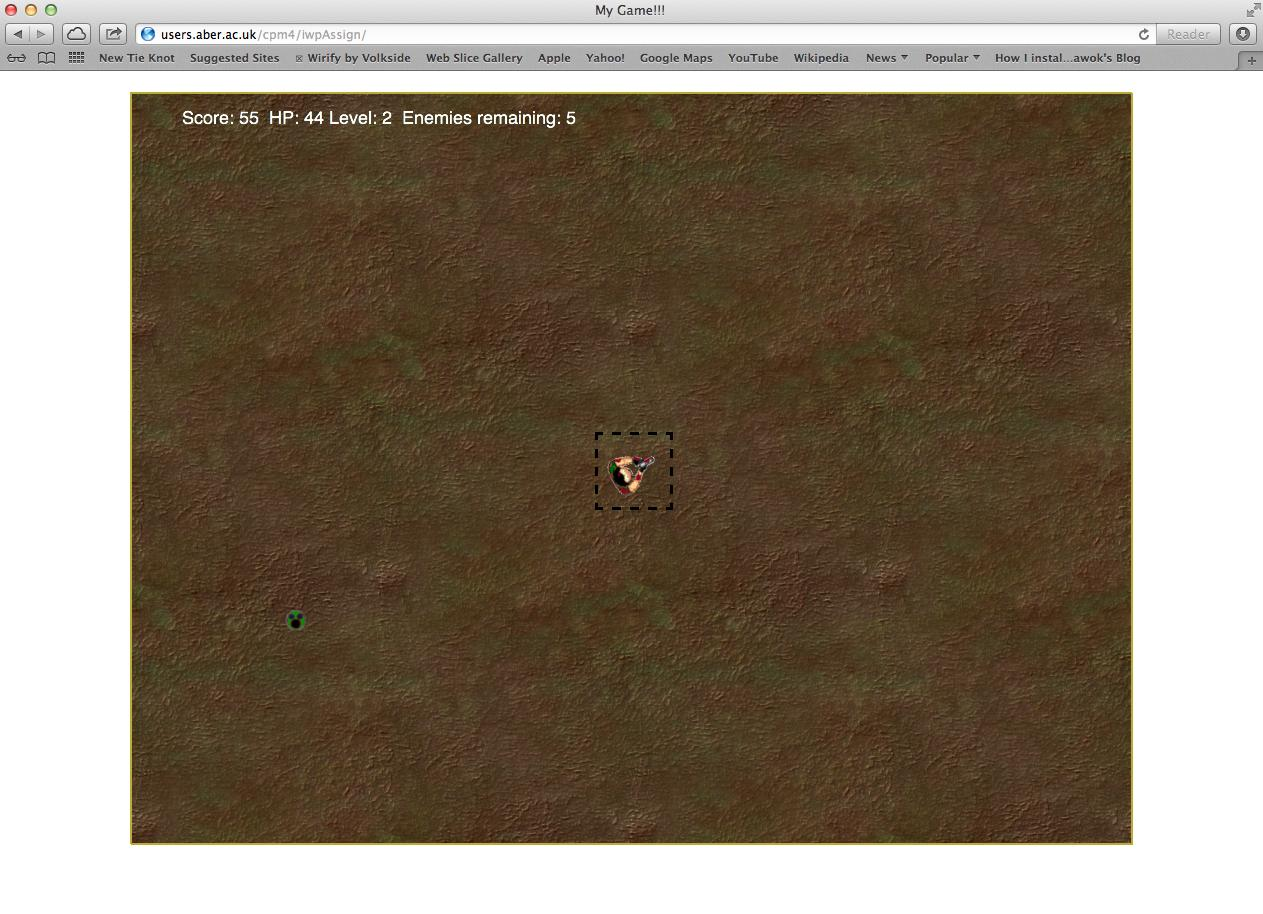
\includegraphics[scale=0.2]{mac.jpg}

\subsection{Windows}
For Firefox and Chrome on Windows the game worked perfectly. However, on IE8 for Windows 7 the eventListeners did not work causing a complete game failure. The game is therefore unplayable ong IE8. 


\section{Reflections and Future Work}
There are many ways in which the game can be improved, the first and most important would be to use a library to help improve overall code. The second would be to improve the gameplay giving it differing enemies and even a story mode and survival mode.
\\\\
I would have liked to get the player movement working so the player wasn't stuck in the middle of the screen and could roam over the level and collect power ups. This would add extended gameplay. Seeing how addictive and well it performed on an Android smart phone it could work out advantagous in being a mobile application.
\\\\
If the game got up to a reasonable standard then it could be offered for advertisment space. If it got developed for the Android market it could be sold for a few pennies and earn some money.
\\\\
The games overall design could be improved with better graphics and presenting the user with more options. I would have also liked to get some character development in by giving a narative and get the player to be able to customise their name and look.






\end{document}

